\documentclass{article}
\usepackage[utf8]{inputenc}
\usepackage[english]{babel}
\usepackage{amsthm}
\usepackage{amssymb}
\usepackage{mathtools}
\usepackage{enumerate}
\newcommand\tab[1][1cm]{\hspace*{#1}}
\usepackage{graphicx}

\author{Kevin Martin\\ CIS675 - Syracuse University}
\title{Homework 2}

\newtheorem*{claim}{Question}
\renewcommand\qedsymbol{$\blacksquare$} 
\begin{document}
\maketitle
\begin{enumerate}
    \item Question 1
      \begin{enumerate}
    \item \ Pseudocode for an efficient algorithm to find and return majority element:\\
      def majorityFind(c [], size)\\
      candidate = 0, count = 1\\
      for i = 1 to (size - 1) do\\
      \tab if c[candidate] == c[i] then\\
           \tab \tab count++\\
       \tab else\\
        \tab \tab count- -\\
       \tab if count == 0 then\\
         \tab \tab candidate = i\\
          \tab \tab count = 1\\
      return c[candidate]\\

    
    \item Claim: the running time of the proposed algorithm is $O(n)$
      \begin{proof}
        Because the above algorithm only needs one pass (and not recursion),
        we must look to the length of the input $n$. The for loop requires a 
        look at all elements in the list, which is $O(n)$ running time.
        Setting up the variables is constant time, and the equality check 
        (A[i]==A[j]) has already be stated to run in constant time $O(1)$.
        Thus the running time of the algorithm depends entirely on the 
        for loop, and the total running time is $O(n)$, where $n>1$.

      \end{proof}

  \end{enumerate}
    \item Question 2
      \begin{enumerate}
        \item Claim: a directed acyclic graph (DAG) always contains a vertex with indegree 0.
      \begin{proof}
      For a graph to be a DAG, it must have at least one source node. If we assume that every
        node in the graph has an indegree of at least one, then let us start at a given node $v_{1}$.
        We will follow the path to its parent. The parent node will also have an indegree of 
        at least one. We continue this process, until each node has been visited, and we will arrive
        back at $v_{1}$, which would mean the graph is a cycle. This is a contradiction.

      \end{proof}
    \item Claim: any connected undirected graph has $|E|\geq(|V|-1)$
    \begin{proof}
    For a graph to be connected, each vertex must have least one edge. However two vertices can share an
      edge. So between two vertices, there could be one edge. If every vertex only had one edge, the graph 
      would not be connected. So there must be at least one pair of vertices that are connected by a 
      common edge ($|V| - 1$). Therefore, there must be at least as many edges as there are vertices, less the 
      (minimum) one shared edge.
    \end{proof}

      \end{enumerate}

\item Question 3\\\\
  \begin{enumerate}
  \item The adjacency matrix representation:\\
  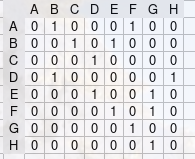
\includegraphics[scale=1]{adjmatrix.png}
  
  \item The adjacency list representation:\\
    $A: B \to F$\\
    $B: C \to E$\\
    $C: D$\\
    $D: B \to H$\\
    $E: D \to G$\\
    $F: E \to G$\\
    $G: F$\\
    $H: G$
    
    \item Table for intermediate visited, pre, and post values of all nodes:\\
    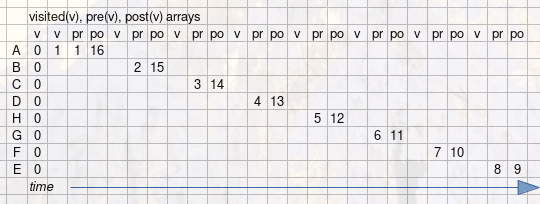
\includegraphics[width=\textwidth]{inttable.png}\\
    \pagebreak
    \item Final DFS tree:\\
    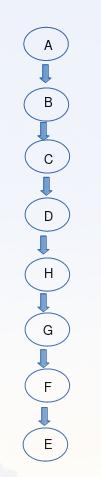
\includegraphics[scale=1]{dfstree.png}


  \end{enumerate}
\pagebreak
\item Question 4\\\\
  Pseudocode of an efficient algorithm to take in graph G(V, E), represetned by an adjacency list,
    and two vertices $x, y \in V$, where the output is the different paths from $x$ to $y$ in G:\\\\
    //wrapper function to set empty path\\
    def diffPathsWrap(x, y, G)\\
    for i = 1 to (size-1) do\\
    \tab visited[i] = False\\     
    \tab path = [] //empty array for each path\\
    diffPaths(x, y, G, path)\\\\

    def diffPaths(x,y, visited, path)\\
    visited[x]=True\\
    if x == y\\
    \tab return path\\
    else\\
    \tab for j in G[x] do\\
    \tab \tab if visited[j] == False\\
    \tab \tab \tab return diffPaths(x, y, visited, path)\\
   \tab \tab path[j].remove //remove current vertex from path\\
   \tab \tab visited[j] = False

\item Question 5\\
  \begin{enumerate}
      \item The order of the strongly connected componets is:\\
        $A \to B \to E$\\
        $C$\\
        $D \to H \to F \to I \to H \to D$
      \item The source SCC is $A \to B \to E$ and the sink SCC 
        is $D \to H \to F \to I \to H \to D$\\
        \pagebreak
      \item Metagraph:\\
      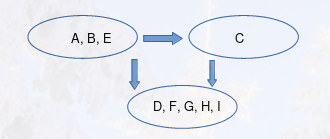
\includegraphics[width=\textwidth]{metagraph.png}
      \item The minimum number of edges one must add to make the graph 
        strongly connected is just one: from $D \to G$. If that edge were
        added, then we could get to any vertex from any other.


  \end{enumerate}
\end{enumerate}
\end{document}


